In diesem Unterkapitel wird der Targetdatensatz deutlich verkleinert und hat dann nur noch 240 Datensamples. Es werden dieselben Tests wie 
im vorherigen Unterkapitel durchgeführt. 

% Es wird zuerst angefangen mit Deep Cascade, da es Unterschiede zwischen den beiden Kaskadenversionen gibt. 
% Bei wenigen Targetdaten gibt es einen Unterschied zwischen Deep Cascade und Direct Cascade. Beides läuft zwar etwas schlechter als mit vielen 
% Daten ist aber mit TF unter Umständen besser als ohne. Dabei ist Deep Cascade etwas besser als Direct Cascade. 

\begin{figure}[htpb]
    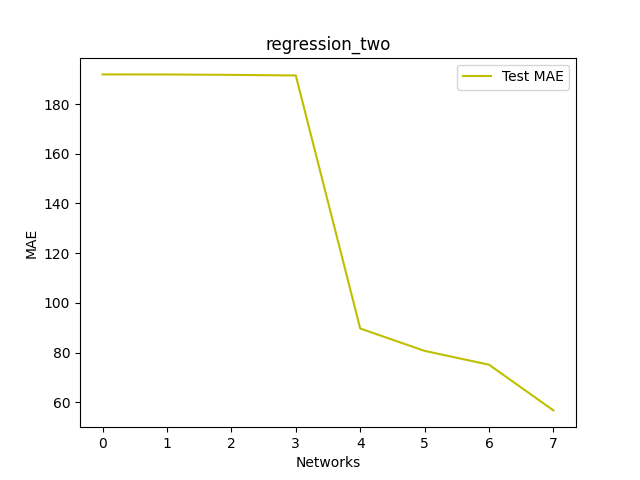
\includegraphics[height=5cm]{../../Plots/ba_plots/regression_small/regr2_ts.png}
    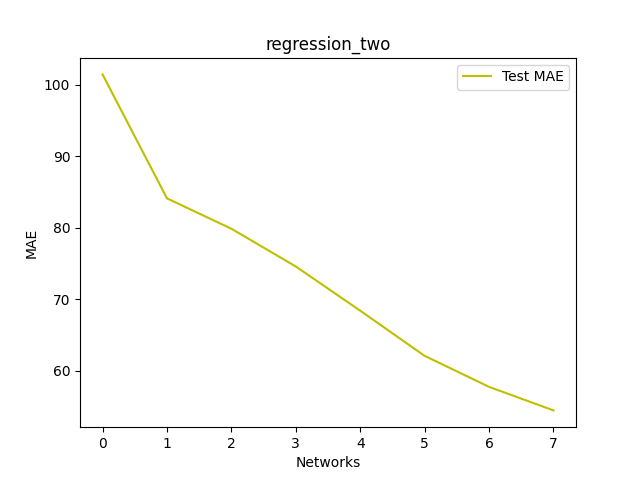
\includegraphics[height=5cm]{../../Plots/ba_plots/regression_small/woregr2_ts.png}
    \caption{\label{fig:smallregr} Vergleich RegressionTwo Netzwerk}
\end{figure}


In Figure 5.4 sind die Ergebnisse des Deep Cascade Netzwerks. Es ist ohne TF tatsächlich besser als mit. Dies liegt daran, dass die Gewichte der 
ersten Hälfte des Netzes nur auf dem Sourcedatensatz passend gelernt haben. 

Es gibt aber deutliche Unterschiede zu Direct Cascade, weshalb beide Netze hier gezeigt werden. 

\begin{figure}[htpb]
    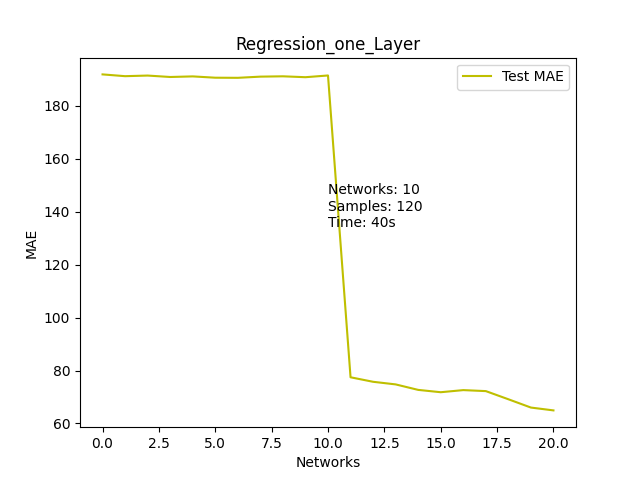
\includegraphics[height=5cm]{../../Plots/ba_plots/regression_small/onelayer_ts.png}
    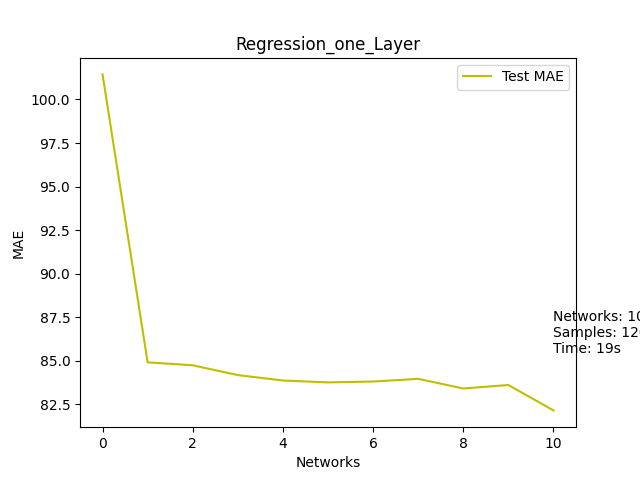
\includegraphics[height=5cm]{../../Plots/ba_plots/regression_small/woonelayer_ts.png}
    \caption{\label{fig:smallonl} Vergleich OneLayer Netzwerk}
\end{figure}

Figure 5.5 bezieht sich auf das Direct Cascade Netzwerk. Es wird deutlich, dass in dieser Kaskadierungsvariante das Netz deutlich schlechter 
ohne TF ist als mit. Die liegt daran, dass das TF über den Augmented Vector als veränderten Input funktioniert und nicht über Gewichte, die 
von dem Sourcedatensatz fertig gelernt worden sind. Allerdings ist das Deep Cascade Netzwerk trotzdem besser. Dies kann aber auch 
an dem dahinter liegenden Netz liegen, da sie nicht nur die gleichen Layer haben. Noch besser ist die Variante, 
die weder Kaskadierung noch TF nutzt, wie in Figure 5.6 gezeigt. 

% Wieso ist die komplette Version trotz der wenigen Daten besser?
\begin{figure}
    \centering
    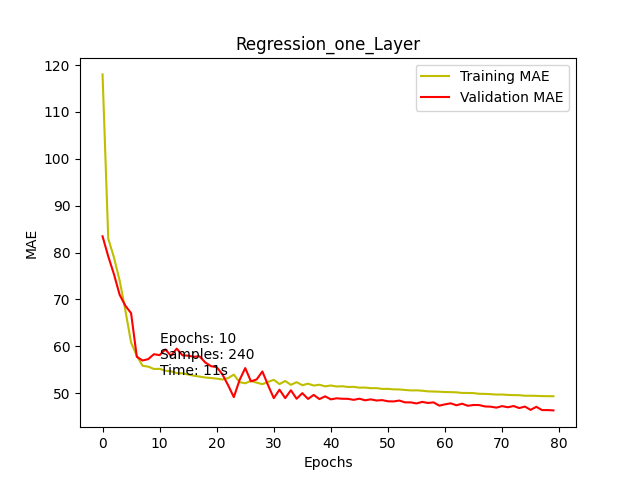
\includegraphics[height=5cm]{../../Plots/ba_plots/regression_small/onelayer_complete.png}
    \caption{\label{fig:smallonlcomp} Komplettes OneLayer}
\end{figure}

Der MAE-Wert der Testdaten beläuft sich hier auf 53 Tausend Dollar, während dieser sonst bei so wenig Datensamples bei 60 bis 80 liegt. 
